
% Inbuilt themes in beamer
\documentclass[aspectratio=169]{beamer}
\usepackage{graphicx}
% Theme choice:
\usetheme{CambridgeUS}

% Title page details: 
\title{Time Series} 
\author{John Green}
\date{April 2024}


\begin{document}

% Title page
\begin{frame}
    \titlepage 
\end{frame}

% Outline frame
\begin{frame}{Outline}
    \begin{enumerate}
       \item Notes on macroeconomic data
       \item Applications
       \item Lags
       \item Autocovariance and autocorrelation
       \item Forecasting
    \end{enumerate}
\end{frame}

\begin{frame}{Macroeconomic data}
    \begin{itemize}
       \item Volatility clustering
       \item Seasonal adjustments
       \item Data revisions and sources
       \item Unemployment rate 
       \item Labor force participation rate 
    \end{itemize}
\end{frame}

\begin{frame}{Uses of time series econometrics}
    Time series analysis is a highly valuable skill in industry:
    \begin{itemize}
       \item Forecasting (eg interest rates, returns to a stock, GDP growth)
       \item Dynamic treatment effects: impact of a policy after 1 month, 3 months, 2 years...
       \item Dynamic system analysis
    \end{itemize}
    But, we will have to deal with problems like correlation over time.
\end{frame}

\begin{frame}{Time series data}
    \begin{itemize}
       \item Generally similar to panel data, but with only one unit
       \item Takes the form $\{Y_t\}_{1 <= t <= T}$ with covariates $\{X_t\}_{1 <= t <= T}$
       \item For now, we assume timing is evenly spaced and there are no missing periods
    \end{itemize}
\end{frame}

\begin{frame}{Lags}
    \begin{itemize}
        \item Lags are very important in time series analysis
        \item $X_{t-1}$ is often a very good predictor of $X_{t}$
        \item More generally, the $j^{\text{th}}$ lag of $Y_t$ is $Y_{t-j}$
        \item We might take a difference: $\Delta_j Y_t = Y_{t} - Y_{t-j}$
    \end{itemize}
\end{frame}

% Outline frame
\begin{frame}{Log variables}
    \begin{itemize}
       \item Oftentimes we will use \textit{log} variables instead of the raw values
       \item Two benefits:
       \begin{itemize}
        \item Makes exponential growth linear
        \item Differences in logs are (approximately) equal to the percentage change:
        $$
        \log(1 + \alpha) \approx \alpha
        $$
        So long as $\alpha$ is ``small''
        \item So, $\log X_{t} - \log X_{t-1} = \log \dfrac{X_{t}}{X_{t-1}}$ is roughly the percentage change in $X$ from $t-1$ to $t$
       \end{itemize}
    \end{itemize}
\end{frame}

\begin{frame}{Autocorrelation}
    \begin{itemize}
       \item Just like with panel data, we will often have correlation between lagged values
       \item First autocovariance of $Y_t$: $cov(Y_t,Y_{t-1})$
       \item First autocorrelation of $Y_t$: $corr(Y_t,Y_{t-1}) \equiv \rho_1$
       \item Can calculate for any lag $j$ in the same way and get the $j^{th}$ serial correlation coefficient
    \end{itemize}
\end{frame}

\begin{frame}{Forecasting and stationarity}
    \begin{itemize}
       \item We will often be interested in making an out-of-sample (OOS) forecast of our variable
       \item This is similar to what we did before trying to target the oracle prediction
       \item We no longer care about causal interpretation of coefficients, OVB, etc.; we just want to get an accurate OOS prediction
       \item This requires that our data be \textit{stationary} (or jointly stationary)
       \begin{itemize}
        \item Intuitively, our out-of-sample data needs to be similar to our sample Data
        \item Technically, we need the joint distribution across time to be independent of the time period we are looking at
       \end{itemize}
    \end{itemize}
\end{frame}

\begin{frame}{Forecasting error}
    \begin{itemize}
       \item An $s$ periods ahead forecast, using estimated coefficients based on $t = 1 , \dots, T$, is:
       $$
        \hat{Y}_{T+s|T}
       $$
       \item The forecast error is:
        $$
        Y_{T+s} - \hat{Y}_{T+s|T}
        $$
        \item And we might evaluate our model based on the mean squared forecasting error:
        $$
        MSFE  = \mathbb{E} \left[ \left( Y_{T+s} - \hat{Y}_{T+s|T} \right)^2 \right]
        $$
    \end{itemize}
\end{frame}

\begin{frame}{Autoregression}
    \begin{itemize}
       \item Regress $Y_t$ on its past (lagged values)
       \item $p^{th}$ order autoregression is $Y_t$ on $Y_{t-1}, \dots, Y_{t-p}$, denoted AR(p):
       $$
        Y_t = \beta_0 + \beta_1 Y_{t-1} + \dots + \beta_p Y_{t-p} + u_t
       $$
       \item Not causal!
       \item Can easily test of value in period $t-s$ is useful with t-test or multiple periods with F-test
       \item For the AR(1) model $Y_t = \beta Y_{t-1} + u_t$, where $| \beta | <1$ and $u = 0$, covariance and correlation between $t$ and $t-s$ are easy:
       $$
        \text{corr} (Y_t, Y_{t-s}) = \beta^s
       $$
    \end{itemize}
\end{frame}

\begin{frame}{Moving averages}
    \begin{itemize}
        \item Moving average model:
        $$
         Y_t = \epsilon_t + \theta \epsilon_{t-1}
        $$
       \item Make substitutions:
       $$
        Y_t = \epsilon_t + \theta \epsilon_{t-1} + \theta^2 \epsilon_{t-2} + \dots
       $$
       \item Some nice properties:
       \begin{itemize}
        \item $Var(Y_t) = \sigma^2 ( 1 +\theta^2)$
        \item $cov(Y_t, Y_{t-1}) = \theta \sigma^2$
        \item $cov(Y_t, Y_{t-j}) = 0 ~~ \forall j>0$
    \end{itemize}
        \item unfortunately, we can't estimate with OLS; have to use NLS
        \item Box-pierce test for serial correlation: $H_0$ is the series is white noise
    \end{itemize}
\end{frame}


\begin{frame}{Covariates}
    \begin{itemize}
       \item We can add in other variables (and their lags) to form an autoregressive distributed lag (ADL) model:
       $$
       Y_t = \beta_0 + \beta_1 Y_{t-1} + \dots + \beta_p Y_{t-p} + \beta_1 X_{t-1} + \dots + \beta_p X_{t-r} + u_t
      $$
      $p$ lags of $Y$ and $r$ lags of $X$, $ADL(p,r)$.
    \end{itemize}
\end{frame}

\begin{frame}{Forecast error}
    \begin{itemize}
       \item Sometimes we look at the root mean squared forecast error, which gives us a ``typical'' error:
       $$
        RMSFE = \sqrt{E\left[\left(Y_{T+1}-\hat{Y}_{T+1 \mid T}\right)^2\right]}
       $$
       \item Three methods for estimating the MSFE:
       \begin{enumerate}
        \item If number of regressors is small, use the in-sample regression error, $\widehat{M S F E}_{S E R}=s_{\hat{u}}^2=\frac{S S R}{T-p-1}$ which ignores the uncertainty from $\hat{\beta}$ 
        \item If errors are homoscedastic, we can use this approximation for the full MSFE:
        $$
        \widehat{M S F E}_{F P E}=\left(\frac{T+p+1}{T}\right) s_{\hat{u}}^2=\left(\frac{T+p+1}{T-p-1}\right)\left(\frac{S S R}{T}\right)
        $$
        \item Method with fewest assumptions: pseudo out of sample. Create a rolling estimate through $t=s$, calculate error for $t=s+1,\dots,T$, repeat; $\widehat{M S F E}_{\text {POOS }}=\frac{1}{P} \sum_{s=T-P+1}^T \tilde{u}_s^2$
       \end{enumerate}
    \end{itemize}
\end{frame}

\begin{frame}{Number of lags}
    \begin{itemize}
       \item How can we choose number of lags $p$?
       \item We can use a bunch of $t$ or $F$ tests... but model will usually be too large
       \item \textit{Information criterion} helps us select by allowing more bias but lower variance (kind of like with the shrinkage estimators)
       $$
       \begin{aligned}
        & \operatorname{AIC}(p)=\ln \left(\frac{\operatorname{SSR}(p)}{T}\right)+(p+1) \frac{2}{T} \\
        & \operatorname{BIC}(p)=\ln \left(\frac{\operatorname{SSR}(p)}{T}\right)+(p+1) \frac{\ln T}{T}
        \end{aligned}
       $$
       \item BIC is consistent; AIC is not but may be good if you think more lags are more important
       \item Can generalize to ADL model
    \end{itemize}
\end{frame}

\begin{frame}{Misc. forecast topics}
    \begin{itemize}
        \item Forecast evaluation
        \item Combining forecasts
        \item Vector autoregression (VAR):
        $$
        \begin{aligned}
            & Y_t=\beta_{01}+\beta_{11} Y_{t-1}+\ldots+\beta_{1 p} Y_{t-p}+\gamma_{11} X_{t-1}+\ldots+\gamma_{1 p} X_{t-p}+u_{1 t} \\
            & X_t=\beta_{02}+\beta_{21} Y_{t-1}+\ldots+\beta_{2 p} Y_{t-p}+\gamma_{21} X_{t-1}+\ldots+\gamma_{2 p} X_{t-p}+u_{2 t}
            \end{aligned}
        $$
        \item Granger causality
        \item Direct vs. iterative prediction
    \end{itemize}
\end{frame}


\begin{frame}{Asset returns}
    \begin{itemize}
        \item Two features:
        \begin{enumerate}
            \item Volatility clustering
            \item Fat tails
        \end{enumerate}
        \item ARCH model:
        $$
        \begin{aligned}
            & Y_t=\mu+u_t \\
            & u_t \sim N\left(0, \sigma_t^2\right) \\
            & \sigma_t^2=\alpha_0+\alpha_1 u_{t-1}^2
            \end{aligned}
        $$
        \item Generalized ARCH (GARCH):
        $$
        \sigma_t^2=\alpha_0+\alpha_1 u_{t-1}^2+\phi_1 \sigma_{t-1}^2
        $$
        \item These capture both of our desired features
    \end{itemize}
\end{frame}

\begin{frame}{Stationarity}
    \begin{itemize}
        \item All these models are assuming \textit{stationarity}
        \item First threat is a \textit{trend}, a persistent long-term movement which might be deterministic or stochastic
        \begin{itemize}
            \item $Y_t = \beta_0 + Y_{t-1} + u_t$ where $u_t$ is serially correlated and $\beta_0$ gives the drift
        \end{itemize}
        \item If $Y_t$ is a random walk, then $\Delta Y_t$ is stationary
        \item Trends may cause:
        \begin{enumerate}
            \item Coefficients biased to 0; bad forecast
            \item t-test doesn't work
            \item Spurious correlation between 2 random walks
        \end{enumerate}
    \end{itemize}
\end{frame}

\begin{frame}{Dickey-Fuller Test}
    \begin{itemize}
        \item Dickey-Fuller test has $H_0$ of random walk vs. $H_A$ of stationarity
        \item Use DF table for critical value
        \begin{itemize}
            \item Depends if model has intercept only or also has a time trend
        \end{itemize}
        \item If DF fails to reject and has a unit root, use first differences model 
    \end{itemize}
\end{frame}


\begin{frame}{Breaks}
    \begin{itemize}
        \item Second threat are structural breaks where the model itself (coefficients) changes over time
        \item If we suspect a break at a specific point we can test this using dummies for before and after the break
        $$
        \begin{aligned}
            Y_t=\beta_0 & +\beta_1 Y_{t-1}+\delta_1 X_{t-1} \\
            & +\gamma_0 D_t(\tau)+\gamma_1\left[D_t(\tau) \times Y_{t-1}\right]+\gamma_2\left[D_t(\tau) \times X_{t-1}\right]+u_t
            \end{aligned}
        $$
        \item Use a Chow test statistic on $\bf{\gamma}$
        \item If we don't know when the break happens we can test dates on $\underline{t} <= t <= \bar{t}$ and take the largest Chow statistic (QLR statistic)
        \item The more QLR stats we compute, the larger the critical value
    \end{itemize}
\end{frame}

% \begin{frame}
%     \centering
%     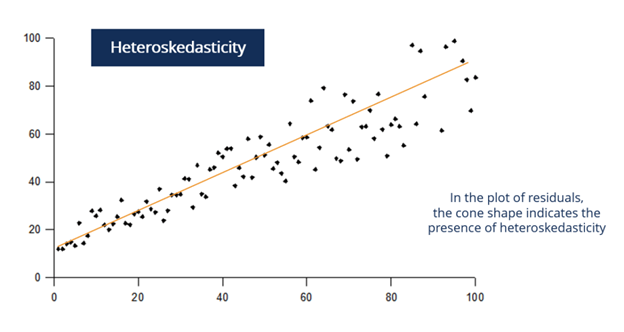
\includegraphics[width = .75\textwidth,keepaspectratio]{./figs/heteroskedasticity.png}
% \end{frame}

\end{document}